\documentclass[american]{article}
\usepackage{titlesec}
\usepackage{graphicx}
\graphicspath{ {images/} }
\usepackage[utf8]{inputenc}
\usepackage{placeins}
%\usepackage[T1]{fontenc}
\usepackage[margin=1in]{geometry}
\usepackage{etoolbox}
\usepackage{xifthen}
\usepackage{ltablex, multirow, makecell, booktabs, caption}
\usepackage[hidelinks]{hyperref}
\usepackage{xcolor}
\hypersetup{
	colorlinks,
	linkcolor={red!50!black},
	citecolor={blue!50!black},
	urlcolor={blue!80!black}
}
%\usepackage{imakeidx}
\usepackage{makeidx}
\makeindex
\usepackage[nottoc]{tocbibind}
\usepackage{babel}
\usepackage{csquotes}
\usepackage[style=ieee,indexing,backref]{biblatex}
\addbibresource{main.bib}
\usepackage{aas_macros}
\usepackage[toc]{glossaries}
\makeglossaries


\titleclass{\subsubsubsection}{straight}[\subsection]

\newcounter{subsubsubsection}[subsubsection]
\renewcommand\thesubsubsubsection{\thesubsubsection.\arabic{subsubsubsection}}
\renewcommand\theparagraph{\thesubsubsubsection.\arabic{paragraph}} % optional; useful if paragraphs are to be numbered

\titleformat{\subsubsubsection}
  {\normalfont\normalsize\bfseries}{\thesubsubsubsection}{1em}{}
\titlespacing*{\subsubsubsection}
{0pt}{3.25ex plus 1ex minus .2ex}{1.5ex plus .2ex}

\makeatletter
\renewcommand\paragraph{\@startsection{paragraph}{5}{\z@}%
  {3.25ex \@plus1ex \@minus.2ex}%
  {-1em}%
  {\normalfont\normalsize\bfseries}}
\renewcommand\subparagraph{\@startsection{subparagraph}{6}{\parindent}%
  {3.25ex \@plus1ex \@minus .2ex}%
  {-1em}%
  {\normalfont\normalsize\bfseries}}
\def\toclevel@subsubsubsection{4}
\def\toclevel@paragraph{5}
\def\toclevel@paragraph{6}
\def\l@subsubsubsection{\@dottedtocline{4}{7em}{4em}}
\def\l@paragraph{\@dottedtocline{5}{10em}{5em}}
\def\l@subparagraph{\@dottedtocline{6}{14em}{6em}}
\makeatother

\setcounter{secnumdepth}{4}
\setcounter{tocdepth}{4}


\newglossaryentry{read}{
	name=Read,
	description={Indicates a source I need to read}
}

\newglossaryentry{categorize}{
	name=Categorize,
	description={Indicates a source I need to categorize}
}

\newglossaryentry{complete}{
	name=Complete,
	description={Indicates a section I need to complete}
}

\newglossaryentry{needcite}{
	name={Needs Citation},
	description={Indicates a claim or which I need to find a citation}
}

\newglossaryentry{expand}{
	name={Expand},
	description={Indicates a bit of information or part of a section which needs expansion to its own section}
}

\newglossaryentry{readmore}{
	name={Read More},
	description={Indicates a citation which I read parts of but which I may need to read more.}
}

\newglossaryentry{morecites}{
	name={More Cites},
	description={Indicates a citation which I have read at least some of which contains more references which are good for reproducibility but which some have not yet made it into the main bibliography. Score this article for the citations.}
}

\newcommand{\Read}{
	\gls{read}
}

\newcommand{\categorize}{
	\gls{categorize}
}

\newcommand{\complete}{
	\gls{complete}
}

\newcommand{\needcite}{
	\gls{needcite}
}

\newcommand{\expand}{
	\gls{expand}
}

\newcommand{\readmore}{
	\gls{readmore}
}

\newcommand{\morecites}{
	\gls{morecites}
}

\newcommand{\ifempty}[3]{%
	\ifthenelse{\isempty{#1}}{#2}{#3}%
}

%\DeclareCiteCommand{\cite}
%  {\bibopenbracket\usebibmacro{prenote}}
%  {\usebibmacro{citeindex}%
%   \printtext[bibhyperref]{\usebibmacro{cite}}}
%  {\multicitedelim}
%  {\usebibmacro{postnote}\bibclosebracket}
%
%\DeclareCiteCommand*{\cite}
%  {\bibopenbracket\usebibmacro{prenote}}
%  {\usebibmacro{citeindex}%
%   \printtext[bibhyperref]{\usebibmacro{citeyear}}}
%  {\multicitedelim}
%  {\usebibmacro{postnote}\bibclosebracket}
%
%\DeclareCiteCommand{\parencite}[\mkbibparens]
%  {\usebibmacro{prenote}}
%  {\usebibmacro{citeindex}%
%    \printtext[bibhyperref]{\usebibmacro{cite}}}
%  {\multicitedelim}
%  {\usebibmacro{postnote}}
%
%\DeclareCiteCommand*{\parencite}[\mkbibparens]
%  {\usebibmacro{prenote}}
%  {\usebibmacro{citeindex}%
%    \printtext[bibhyperref]{\usebibmacro{citeyear}}}
%  {\multicitedelim}
%  {\usebibmacro{postnote}}
%
%\DeclareCiteCommand{\footcite}[\mkbibfootnote]
%  {\usebibmacro{prenote}}
%  {\usebibmacro{citeindex}%
%  \printtext[bibhyperref]{ \usebibmacro{cite}}}
%  {\multicitedelim}
%  {\usebibmacro{postnote}}
%
%\DeclareCiteCommand{\footcitetext}[\mkbibfootnotetext]
%  {\usebibmacro{prenote}}
%  {\usebibmacro{citeindex}%
%   \printtext[bibhyperref]{\usebibmacro{cite}}}
%  {\multicitedelim}
%  {\usebibmacro{postnote}}
%
%\DeclareCiteCommand{\textcite}
%  {\boolfalse{cbx:parens}}
%  {\usebibmacro{citeindex}%
%   \printtext[bibhyperref]{\usebibmacro{textcite}}}
%  {\ifbool{cbx:parens}
%     {\bibcloseparen\global\boolfalse{cbx:parens}}
%     {}%
%   \multicitedelim}
%  {\usebibmacro{textcite:postnote}}

\DeclareCiteCommand{\citejournalorbooktitle}
  {\usebibmacro{prenote}}
  {\usebibmacro{citeindex}%
    \iffieldundef{journaltitle}{\usebibmacro{booktitle}}{\usebibmacro{journal}}}
  {\multicitedelim}
  {\usebibmacro{postnote}}

\DeclareFieldFormat[legislation]{title}{#1}
\renewcommand*{\postnotedelim}{
  \ifentrytype{legislation}
    {\addspace}
    {\addcomma\space}
}

\newenvironment{refdef}[2] {
	\noindent \textbf{\citetitle{#1}} \cite{#1}\\ \citejournalorbooktitle{#1} \textit{(\citeyear{#1})}\\ \texttt{#2} \vspace{0.2in} \par
} {
\vspace{0.2in}
}

\title{Reproducibility Notes}
\author{NCSA Reproducibility Group}
\date{\today}

\begin{document}

\maketitle

\tableofcontents

\section{Contributors} \label{sec:contributors}

This document contains work from the NCSA Reproducibility group. The contributors are listed below.

\begin{itemize}
\item Matthew Krafczyk
\item Adhithya Bhaskar
\end{itemize}

\section{Introduction} \label{sec:introduction}

These are my research notes while working at NCSA.

\complete

\section{Reproducibility Terms} \label{sec:reproducibility-terms}

I will be using the ACM terms for reproducibility \cite{acm-badging}. In order of increasing strength or rigor they are:

\begin{itemize}
\item \textbf{Repeatability}: When a research team can get the same conclusions using the same experimental methods as previous
\item \textbf{Replicability}: When a separate research team can get the same conclusions using the same experimental methods as previous
\item \textbf{Reproducibility}: When a separate research team can get the same conclusions using a different experimental method as previous
\end{itemize}

There is some contention about these terms, I believe the biology people use different terms. \needcite

\section{Reproducibility Issues} \label{sec:reproducibility-issues}

Here I'm trying to collect all the different issues which exist with reproducibility. I'm using it as a space to make sense of these issues as well as collect the references which make the case.

\complete

\subsection{Sociological Issues} \label{sec:repro-sociological-issues}

\begin{itemize}
\item Scrutinization
\item Competitive Advantage
\item Licensing
\item Monolithic codebases
\item Dirty code
\item \textbf{Some seem \textit{strange} given the published article}
\end{itemize}

\complete

\subsection{Software Issues} \label{sec:repro-software-issues}

\begin{itemize}
\item Numerical error
\item Transparent machine software/hardware failures
\item Hard-coded machine topologies
\item \textbf{Some of these are \textit{unavoidable}}
\end{itemize}

\complete

\subsection{Hardware Issues} \label{sec:repro-hardware-issues}

\begin{itemize}
\item Special hardware requirements
\item Silent Failures
\item \textbf{Some of these are \textit{unavoidable}}
\end{itemize}

\complete

\subsubsection{Specialized Hardware} \label{sec:repro-spec-hardware}

Here I'm detailing various specialized hardware I hear about which might hamper reproducibility efforts.

\begin{itemize}
\item Large Supercomputer (for large computing runs)
\item GPUs (Usually not hard to get, but still an obstacle)
\item FPGA
\item Neuromorphic Chips \cite{neuromorphic-chips-webarticle}
\item TPUs \cite{jouppi-tpu-performance-2017}
\end{itemize}

\complete

\subsubsection{Handling specialized hardware} \label{sec:repro-spec-hardware-handling}

Results run on specialized hardware should still be replicable as long as an appropriate virtual machine or emulator is available for that architecture.

\complete

\subsection{Compatibility Issues} \label{sec:repro-compatibility-issues}

DOES THIS SUBSECTION DESERVE ITS OWN SECTION??

Study compatibility is a serious problem which prevents the comparison of scientific studies when researchers do not agree on input formatting, output formatting, and general scientific workflow. Without this compatibility, major work must be done to allow apples to apples comparisons between scientific works.

To make matters worse, allowing scientists to steal a method from another scientist and use it in their IDE is currently impossible due to incompatibilities inherent in each application's assuredly divergent development lines. Thus solving the compatibility will be a great step forward towards allowing the three currently difficult workflows.

\complete

\section{Reproducibility Scandals} \label{sec:reproducibility-scandals}

Here, I'm going to collect together known scandals arrising from the lack of reproducibility.

\subsection{Medicine} \label{sec:scandals-medicine}

Medicine specific scandals

\begin{itemize}
\item 2004 GlaxoSmithKline Paxil uneffective \cite{dhb-zurich-hp}. \needcite
\item 2011 Bayer could only reproduce 17 of 67 published studies \cite{dhb-zurich-hp}. \needcite
\item 2012 Amgen could only reproduce 6 of 53 published cancer studies \cite{dhb-zurich-hp}. \needcite
\item 2014 Tamiflu review showed only small decrease in some smptoms \cite{dhb-zurich-hp}. \needcite
\item 2017 A doctor who developed a scale for measuring drug regime adherence in patients is extracting licensing fees from users of the scale. This makes reproducing work using said scale more difficult. \cite{marcus-payup-retract-2017}
\end{itemize}

\subsection{Physics} \label{sec:scandals-physics}

Physics specific scandals.

\begin{itemize}
\item BICEP2 Gravitational Wave `discovery' \cite{dhb-zurich-hp}. \needcite
\end{itemize}

\complete

\subsection{Chemistry} \label{sec:scandals-chemistry}

Chemistry specific scandals.

\begin{itemize}
\item Gaussian software banning competitors from using their software
\end{itemize}

\subsubsection{Gaussian} \label{sec:scanals-chemistry-gaussian}

Gaussian Inc. actively bans competing researchers from using their code. This means if you are working on a tool which performs the same tasks as Gaussian and probably especially if you claim to do a better job than Gaussian, you are banned from using Gaussian forever. This means that said researchers cannot validate research published by other scientists who do use the Gaussian software. The website \cite{banned-by-gaussian} goes into great detail about this ongoing crisis. They furthur reference journal standards produced by the Pure and Applied Chemistry journal \cite{pac-guidelines-publication-1998,pac-guidelines-presentation-1998} which make mention of the requirement that sufficient technical details be published to permit the replication of any published article's results. Gaussian banning scientists directly contradicts this stance by the journal.

\complete

\section{Causation of Reproducibility problems} \label{sec:causation}

This section summarizes why reproducibility is a problem in various fields and not other.
\complete

\section{Numerical Precision Issues} \label{sec:precision}

This section summarizes issues related to numerical precisions. Whether it's an algorithm touted to be more precise, or a tool to optimize a program it will be found here.

In calculations which are sensitive to numerical precision, small errors may lead to large numerical problems such as taking the wrong branch in a conditional statement \cite{high-precision-arith-in-science}.

\complete

\subsection{IEEE floating point arithmetic} \label{sec:precision-ieee-float}

Here, I review some properties of the IEEE floating point standard. I may later add some information about some fixed-point or alternative floating point implementations.

The IEEE 754 floating point standard \cite{ieee-754-2008,ieee-754-2008-redline} defines operation and exception details for the floating point number.

Each floating point number consists of a `mantissa' and an `exponent'. The mantissa ($m$) is a signed integer of precision $p$ and the exponent ($e$) is a signed integer with precision $e$. Each floating point number is also defined by a radix($b$) which can either be 2(binary) or 10(decimal). Each floating point number then has a value $m\cdot b^e$. Table \ref{tab:float-par} defines these parameters for each defined binary type.

\FloatBarrier
\begin{table}[t]
	\caption{Floating point variable parameters for each binary (radix 2) defined type. All taken from \cite{ieee-754-2008}.} \label{tab:float-par}
\begin{tabular}{llll}
\hline
bit-width & 32 & 64 & 128 \\
\hline
specification name & binary32 & binary64 & binary128 \\
\hline
colloquial name & \texttt{float} & \texttt{double} & \texttt{quad} \\
\hline
precision & 24 & 53 & 113 \\
\hline
exponent precision & 8 & 11 & 15 \\
\hline
equivalent decimal precision & ~7 digits & ~16 digits & ~34 digits \\
\hline
\end{tabular}
\end{table}
\FloatBarrier

\subsubsection{Normalization} \label{sec:precision-ieee-norm}

A common way of expressing a floating point number is like this: $\pm\beta^e\times. d_1 d_2 \ldots d_t$ with $d_1 \neq 0$ for \textit{normalized} numbers. when $y$ is less than $\beta^{emin}$, $d_1$ cannot be non-zero and so we have sub-normal numbers \cite{higham-numerical-accuracy-and-stability}.

\subsubsection{Rounding modes} \label{sec:precision-ieee-round}

From libc and ieee \cite{gnu-libc-rounding,ieee-754-2008}, we have four rounding modes. \cite{gnu-libc-rounding} says that fpu calculations occur at higher precision, and then the value is stored in the specified data width where rounding occurs. I haven't found the statement in \cite{ieee-754-2008} which says this.

\begin{itemize}
\item Round to nearest (default)
\item Round to $+\infty$
\item Round to $-\infty$
\item Round to 0
\end{itemize}

\subsubsection{Machine Epsilon} \label{sec:precision-ieee-epsilon}

From lemma 2.1 on page 37 of \cite{higham-numerical-accuracy-and-stability}, The spacing between a normalized floating point number $x$ and an adjacent normalized floating point number is at least $\beta^{-1}\epsilon|x|$ and at most $\epsilon|x|$ \cite{higham-numerical-accuracy-and-stability}. This also means that the largest error between an infinitely precise number, and it's nearest neighbor is $\epsilon/2 = \beta^{-(p-1)}/2$. This value is known as the machine epsilon.

Another definition: Machine epsilon is defined as the smallest number that, when added to one, yields a result different from one. This is $b^{-(p-1)}$ and $\epsilon/2$ for the round-to-nearest procedure.

\subsubsection{Known numerical anomalies} \label{sec:precision-ieee-anomalies}

Bailey goes through a great discussion of known numerical anomalies here \cite{dhb-numerical-bugs}. I'm going to talk about a couple of them.

\begin{itemize}
\item Language-based difficulties
\begin{itemize}
\item code constant translation to lower precision types than those on the rhs of equations.
\item Expression evaluation to the precision of only the operand types and not the type on the rhs of the equation.
\end{itemize}
\item Avoidable Numerical Anomalies
\begin{itemize}
\item Conditional branches with floating-point comparison which may fail to hold
\item error accumulation from summation of small numbers
\end{itemize}
\item Unavoidable Numerical Anomalies
\begin{itemize}
\item Large equations or systems of equations are demanding numerically.
\end{itemize}
\end{itemize}

\subsubsection{Reproducibility Attributes} \label{sec:precision-ieee-attributes}

This section discusses the reproducibility attributes present in the IEEE 754 standard. \cite{ieee-754-2008}

\complete

\subsection{Scientific Problems needing special precision} \label{sec:precision-special}

A number of problems need special scientific precision. David Bailey did a great job laying this out\cite{high-precision-arith-in-science,dhb-zurich-hp}. I reproduce his table from \cite{dhb-zurich-hp} as Table \ref{tab:precision} to give an idea of the gamut.

\FloatBarrier
\begin{table}[t]
\caption{Typical bit precision necessary for various scientific fields}\label{tab:precision}
\begin{tabular}{lr}
Problem Type & Number of bits(?) necessary \\
Planetary orbit calculations & 32 \\
Climate modeling & 32 \\
Optimization problems in biology and other fields & 32\\
Schrodinger solutions for lithium and helium atoms & 32\\
Scattering amplitudes of fundamental particles & 32\\
Discrete dynamical systems & 32\\
Supernova simulations & 32-64 \\
Coulomb n-body atomic system simulations & 32-120\\
Electromagnetic scattering theory & 32-100\\
The Taylor algorithm for ODEs & 100-600\\
Ising integrals from mathematical physics & 100-1,000\\
Problems in experimental mathematics & 100-50,000\\
\end{tabular}
\end{table}
\FloatBarrier

MINOS \needcite software for biochemistry contains precision problems \cite{dhb-zurich-hp}.

\subsection{Solutions to reduction error issues} \label{sec:precision-solutions}

Two techniques which can be used to solve reduction error are to either enforce an ordering to the summation. This can be done by creating a unique id for each element of the sum, and guarenteeing that these ids are identical each run and making sure that the summation sums the id'd elements the same way each time. Another is to use the technique outlined here: \cite{repro-fast-sum}.

There are some techniques to test whether your program has numerical precision difficulties. You can for instance, change the rounding mode. If the program's result varies wildly, you know there is a precision problem, but it does nothing to clear this up \cite{dhb-numerical-bugs}. You can add an adjustable 'fuzz' to a computation to see whether this affects the results offered. This can prove numerical instability \cite{dhb-numerical-bugs}.

\subsection{Software implementing arbitrary precision floating point} \label{sec:precision-arbitrary}

Here I collect packages which implement arbitrary precision floating point arithmetic in various ways. These packages were discovered in \cite{high-precision-arith-in-science}.

\begin{itemize}
\item ARPREC (Arbitrary, pre-set precision level) \needcite
\item DDFUN (double double precision) \needcite
\item FMLIB/FMZM90 (low-level multiple-precision libarary) \needcite
\item GMP (multiple-precision library) \needcite
\item Predicates (Specialized package for computational geometry) \needcite
\item QD (double double and quad double arithmetic. Faster than arbitrary precision libraries when only double double or quad double precision is sufficient) \needcite
\item MPFR/MPFR++ (multi-precision library with exact rounding \needcite
\item MPFUN90 (ARPREC equivalent entirely in fortran90) \cite{mpfun}
\item VPA (arbitrary precision library for fortran) \needcite
\end{itemize}

From \cite{dhb-zurich-hp}, we have:

\begin{itemize}
\item CORVETTE \needcite
\end{itemize}

Using high-precision software increases runtimes. double-double Takes 5 times longer than 64-bit arithmetic, 25 times longer with quad-double, and 50 times for 100-digit arithmetic. Computational cost scales as $p^2$ up to about 1000 digits then costs $p\log p$ if you're using FFT-based multiplication. \cite{high-precision-arith-in-science} (\needcite for FFFT-based multiplication)

\subsection{Program Precision Optimizers} \label{sec:precision-optimizers}

These tools analyze a program's operation in some way and produce recommendations about data types or run conditions which will preserve or increase a program's numerical precision while also improving or largely preserving a programs performance.

\begin{itemize}
\item BLAME Analysis \cite{blame-analysis}
\item PRECIMONIOUS \needcite
\end{itemize}

A few examples of applications which have benefitted from these techniques or detailed studies include climate modelling, supernova simulations, coulomb n-body simulations, studies of the fine-structure constant, E-M scattering theory, vortex sheet roll-up (fluid dynamics) simulations, computational geometry, compuational number theory, experimental math (including the discovery of the BBP $\pi$ formula, quantum field theory (Using PSLQ computations (More info on PSLQ here \cite{dhb-numerical-bugs}) (All of the previous fields are from \cite{high-precision-arith-in-science}).

Ising integrals, tanh-sinh integration algorithm, box-integrals, minimal polynomials, algebraic numbers in poisson potential functions \needcite \cite{dhb-zurich-hp}.

\subsubsection{BLAME Analysis} \label{sec:precision-optimizers-blame}

This tool is created from LLVM and analyzes code passed through it for operations which can be run at reduced precision. \cite{blame-analysis}

\complete?

\subsection{Algorithmic concepts dealing with numerical precision} \label{sec:precision-algorithms}

Condition number, the condition number of a function with respect to an argument measures how much the output value of the function can change for a small change in the input argument. \needcite

\subsection{Theoretical Tools to approach the problem of numerical precision} \label{sec:precision-theory}

Here I go over some theoretical tools to confront numerical precision issues. The idea is that some or all of the ideas in this section can be turned on computational code to produce uncertainty estimates of their results.

\complete

\subsubsection{Interval arithmetic} \label{sec:precision-theory-interval}

This technique focuses on calculating everything with an interval rather than a single number. This way the uncertainty interval is propogated all the way to the end of the calculation. (There is a wiki article but I need to find a real source.) \needcite

Unfortunately, it's runtime cost is enormous \cite{dhb-numerical-bugs}.

\complete

\section{Goals for reproducibility} \label{sec:goals}

I want to make the following methods more easily executable. Replicability and Compatibility will be huge steps towards making this happen.

\complete

\subsection{Method Appropriation} \label{sec:goals-appropriation}

\begin{enumerate}
\item \textbf{A} is working on airfoil using method \boldmath$\alpha$, but sim has a problem
\item \textbf{B} publishes method $\beta$ which claims to fix said problem
\item \textbf{A} reads \textbf{B}'s paper
\item \textbf{A} downloads \textbf{B}'s materials, verifies the result
\item \textbf{A} then uses method $\beta$ to solve their problem
\item \textbf{A} publishes their airfoil citing \textbf{B} as simulation method
\end{enumerate}

\subsection{Method Tweaking} \label{sec:goals-tweaking}

\begin{enumerate}
\item \textbf{A} needs to simulate a large protein to find binding sites
\item \textbf{A} finds method \boldmath$\beta$ by \textbf{B} for simulating large proteins efficiently, but doesn't find binding sites.
\item \textbf{A} download's \textbf{B}'s materials, verifies the result
\item \textbf{A} adds code to find binding sites to $\beta$ producing method $\alpha$
\item \textbf{A} publishes method $\alpha$ citing \textbf{B}'s method $\beta$.
\end{enumerate}

\subsection{Method Improvement} \label{sec:goals-improvement}

\begin{enumerate}
\item Performing lattice QCD, \textbf{A} finds method \boldmath$\beta$ by \textbf{B}.
\item \textbf{A} spots mistake in method $\beta$ from article
\item \textbf{A} downloads \textbf{B}'s materials, verifies the result
\item \textbf{A} changes $\beta$ creating method $\alpha$ solving mistake
\item \textbf{A} runs method $\alpha$ verifying better agreement with experimentally measured values
\item \textbf{A} publishes $\alpha$ citing \textbf{B} about this change
\end{enumerate}

\section{Empirical Reproducibility Studies} \label{sec:empirical}

Here I'm collecting a list of all empirical studies about reproducibility in the scientific community. These are good places to grab statistics to show people how bad the whole situation really is. I'm collecting their timeframe, and what field they cover. See Table \ref{tab:empirical-studies} for the table.

\complete

\FloatBarrier

\begin{tabularx}{\textwidth}{lXllX}
\caption{A list of replicability and reproducibility studies and what they say} \label{tab:empirical-studies} \\
\toprule
Citation & Title & Timeframe & Field & Results \\
\midrule
\endfirsthead
\multicolumn{5}{c}{Table \thetable\enspace (continued)} \\
\toprule
Citation & Title & Timeframe & Field & Results \\
\midrule
\endhead
\bottomrule
\multicolumn{5}{l}{Table \thetable\enspace To be continued...}
\endfoot
\bottomrule
\endlastfoot
\cite{dewald-replication-econ-1986} & \citetitle{dewald-replication-econ-1986} & 1986 & Economics & Response rates to requests for data were higher for articles which were accepted and under review than for articles which were already published (pub: 66\%, acc: 96\%, rev: 75\%), Only 15\% of received data sets were properly documented and cited, 26\% were incomplete \readmore \\
\hline
\cite{hatton-scientific-software-accurate-1994} & \citetitle{hatton-scientific-software-accurate-1994} & 1994 & Geophysics & N-version replication study. Approximate cumulative precision-loss of 1\% every 4000 source lines (about 3000 executable lines) in terms of average absolute difference. \\
\hline
\cite{peng-epidemiologic-2006} & \citetitle{peng-epidemiologic-2006} & 2005 & Epidemiology & 93\% of articles do not detail data processing. 84\% of articles did not release data. \\
\hline
\cite{wicherts-poor-availability-psychology-2006} & \citetitle{wicherts-poor-availability-psychology-2006} & 2006 & Psychology & After generous attempts to get data from published study authors, only these authors were only able to obtain 25.7\% of the datasets in their article cohort. \\
\hline
\cite{arrowsmith-phase-ii-failures-2011} & \citetitle{arrowsmith-phase-ii-failures-2011} & 2011 & Biology & Success rates in Phase II trails have fallen from 28\% to 18\%. As mentioned in \cite{printz-rely-published-2011} \\
\hline
\cite{printz-rely-published-2011} & \citetitle{printz-rely-published-2011} & 2011 & Biology & In only 20-25\% of projects were the relevant published data completely in line with their in-house findings \\
\hline
\cite{Begley2012} & \citetitle{Begley2012} & 2012 & Cell Biology & Only 6 of 53 landmark biotechnology papers held up. \\
\hline
\cite{economics-replicability-fed} & \citetitle{economics-replicability-fed} & 2015 & Economics & 22/67 (33\%) replicated without author contact 29/59 (49\%) replicated with author contact. \\
\hline
\cite{aac4716} & \citetitle{aac4716} & 2015 & Psychology & 97\% of original studies had statistically significant results 36\% of replications had statistically significant results. 47\% of original effect sizes were in the 95\% confidence interval of the replication effect size. 83\% of studies had a larger effect size in the original study. 39\% of effects were subjectively rated to have replicated the original results. Replication success was more consistently related to the original strength of evidence (such as original $P$ value, effect size, and effect tested) than to characteristics of the teams and implementation of the replication (such as expertise, quality, or challenge of conducting the study)\\
\hline
\cite{collberg-repeatability-2016} & \citetitle{collberg-repeatability-2016} & 2016 & Computer Science & 44\% of computer science article authors released their source code. \Read there are others. \\
\hline
\cite{berghmans-survey-open-data-dataset-2017} & \citetitle{berghmans-survey-open-data-dataset-2017} & 2017 & Datascience? & This article contains many good statistics. \Read Here are a few: 73\% of respondants said that having access to others research data benefits or would benefit their own data. Only 65\% of respondants said they had shared their research data with others and only 52\% said that they provide their research data to publishers so it can be made access with their article. An interesting divide. \\
\bottomrule
\end{tabularx}

\FloatBarrier

\section{Reproducibility Software} \label{sec:software}

Here I'm collecting a list of all reproducibility software I have encountered. I'll discuss each in turn hitting what they offer and what they lack. Any specific system which doesn't have it's own section means I haven't tried it or don't know enough about it to say anything.

\complete

\subsection{Containers} \label{sec:software-containers}

\subsubsection{Introduction}

Containers are a method of operating system virtualization that isolate applications including their runtime environment and all the files required to run. LXCs (Linux Containers) are able to run multiple Linux containers on a host with a single kernel. This is done by providing the linux kernel's cgroups feature and isolated namespaces for and isolated environment for containers\cite{containers-hierarchy}.

\begin{figure}[h]
    \centering
    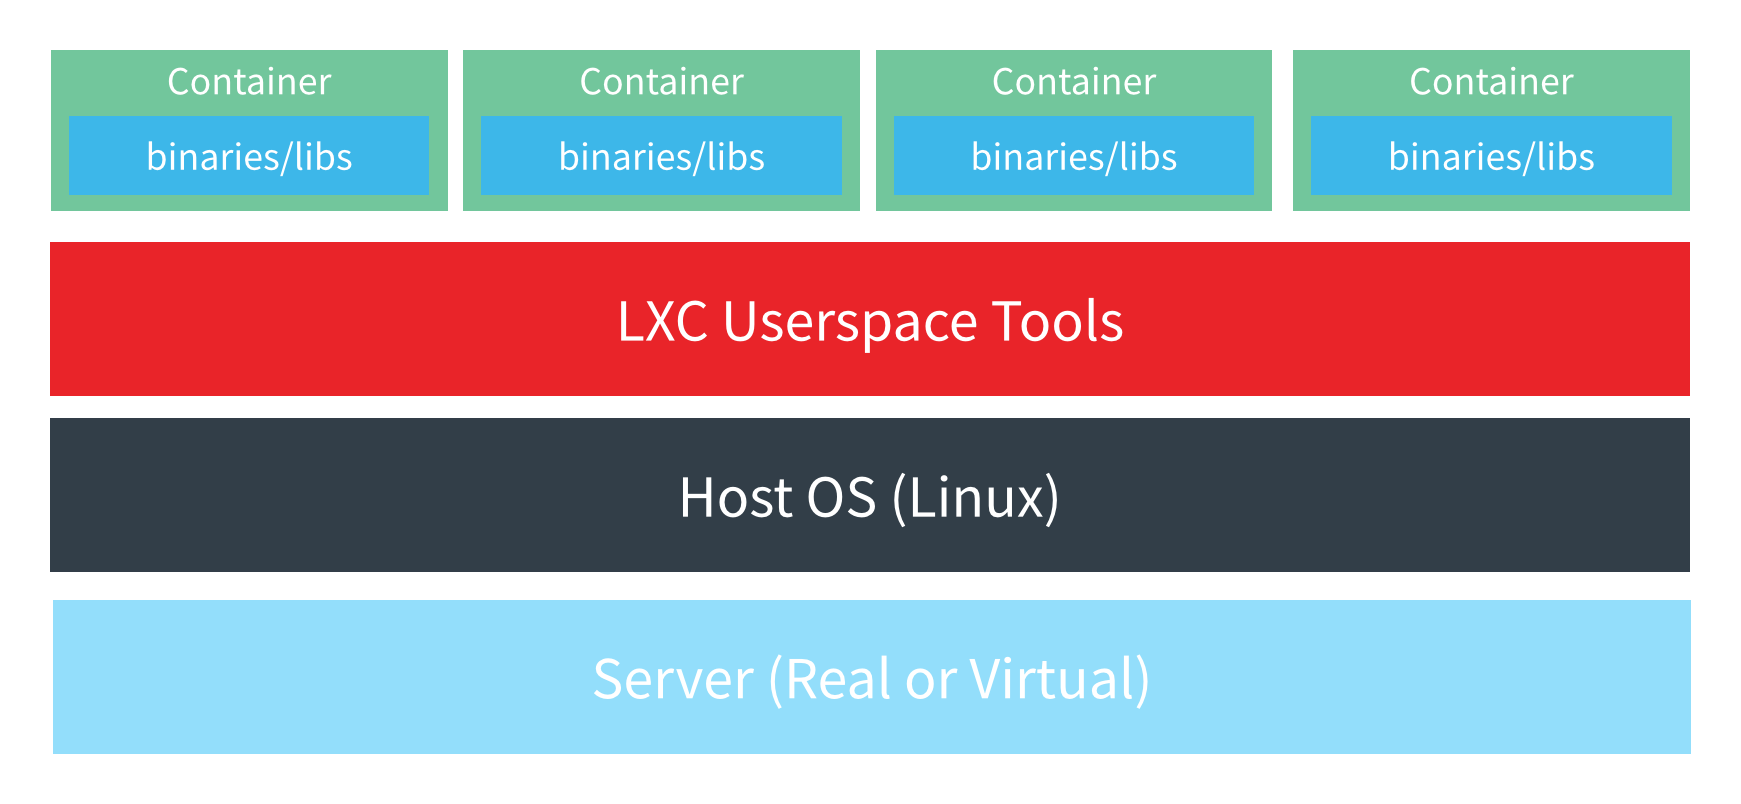
\includegraphics[width=0.75\textwidth]{containers-intro}
    \caption{Figure showing a Linux container stack}
    \label{fig:containers-intro}
\end{figure}

Containers are restricted to Linux since containers need to be able to isolate processes without a new kernel. They run on the host OS's kernel and rely on system calls for processes. This is stable over different kernel versions and hence the host does not need to install a new kernel depending on the container required version\cite{kernel-space-redhat}.

Once an application is compiled, the set of system calls that an application uses is embedded in the binary. Containers don't abstract the need for the user space and kernel space to share a common set of system calls as seen in figure \ref{fig:sys-calls}. In a containerized world, this user space is bundled up and shipped around to different hosts, ranging from laptops to production servers.

\begin{figure}[h]
    \centering
    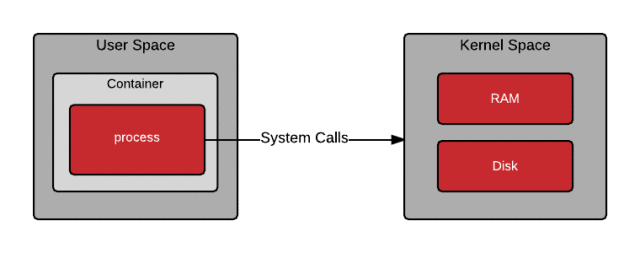
\includegraphics[width=0.75\textwidth]{system-calls}
    \caption{Figure shared system calls}
    \label{fig:sys-calls}
\end{figure}


\subsubsection{chroot system calls}
The chroot system call is a critical foundation for containers.  The chroot mechanism can redefine the root directory for any running program, effectively preventing that program from being able to name or access resources outside that root directory tree. These partitions are referred to as chroot jails\cite{intel-whitepaper}. It redefines the root directory for running a program and prevents the program from viewing resources outside the directory. It shares a single kernel with the host while being tamper-resistant and preventing malicious code to "break out" of the jail.


\subsubsection{cgroups}

cgroups is a Linux kernel feature that allows the user to allocate and monitor resources such as memory, network bandwidth, CPU, disk I/O, etc into hierarchical groups\cite{cgroups-wiki}. Some important features provided by cgroups are\cite{cgroups}:
\begin{itemize}
	\item Resource limiting
	\item Prioritization
	\item Accounting
	\item Control
\end{itemize}

\subsubsection{namespaces}

Namespaces wrap a global system resource into an abstraction that makes it appear to the processes within the namespace to appear to have their own isolated instance of the global resource\cite{namespaces}.

There are currently 6 types of namespaces\cite{namespaces}
\begin{itemize}
	\item Mount namespaces - Mount points
	\item UTS namespaces - Hostname and NIS Domain name
	\item IPC namespaces - System V IPS, POSIX message queues
	\item PID namespaces - Process IDs
	\item Network namespaces - Network devices, ports, etc.
	\item User namespace - User and group IDs
\end{itemize}

\subsubsection{Security}

Initially, in LXCs, the root user of the container could run any code on the host system with complete root access to the host's system. However, since v1.0, multiple security features have been implement to limit access to the host's hardware\cite{lxc-wiki}.

\subsubsubsection{Discretionary Access Control}
It is a method of restricting access to objects based on the identity of subjects and/or groups to which they belong. The controls are discretionary in the sense that a subject with a certain access permission is capable of passing that permission. Based on the filesystem ownership and permissions, the kernel uses discretion to allow access to files\cite{dac}.

\subsubsubsection{Mandatory Access Control}
It is a system wide policy that dictates which who is allowed access to certain files and the permissions cannot be altered by the user unless the MAC policy modified or removed.

\subsubsection{Popular Containerization Software}

\begin{itemize}
\item Docker \cite{Docker}
\item Vagrant \needcite
\item Singularity \cite{Singularity}
\item Kuberneties \needcite
\item Shifter \needcite
\end{itemize}

\complete

\subsection{Virtual Machines} \label{sec:software-virtual}

These techniques use a hypervisor to run a logically separate virtual machine on a host machine. These tend to be slower, but as hardware vendors add support for virtualization technology to their chipsets they are getting closer to native performance.

\begin{itemize}
\item VMWare \needcite
\item Virtual Box \needcite
\item KVM \needcite
\end{itemize}

\complete

\subsection{Research Environments} \label{sec:software-environments}

From \cite{stodden-sharing-reproducibility-talk-2017}.

\begin{itemize}
\item Verifiable Computational Research \needcite
\item knitR \needcite
\item Collage Authoring Environment \needcite
\item Sumatra \needcite
\item Galaxy \needcite
\item SHARE \needcite
\item Sweave \needcite
\item SOLE \needcite
\item GenePattern \needcite
\item torch.ch \needcite
\item Cyverse \needcite
\item Open Science Framework \needcite
\item IPOL \needcite
\item Jupyter \needcite
\item NanoHUB \needcite
\item Vistrails \needcite
\end{itemize}

\subsection{Workflow Managers} \label{sec:software-managers}

These softwares purport to handle all of our scientific workflow needs. They handle your source code, build your application, run it and compile the paper from the results produced. Some workflows may not fit, but they are working hard to make sure that it doesn't stay that way.

\begin{itemize}
\item Popper \cite{popper}
\item WholeTale \Read \categorize \needcite
\item CodeOcean \Read \categorize \needcite
\item Taverna \needcite
\item Kurator \needcite
\item Wings \needcite
\item Kepler \needcite
\item Pegasus \needcite
\item Everware \cite{everware}
\item CDE \needcite
\item binder.org \needcite
\item NextFlow \needcite
\item Common Workflow Language \needcite
\item revisit \cite{matloff-revisit-2017}
\end{itemize}

\subsubsection{Popper} \label{sec:software-managers-popper}

Popper \cite{popper} is an interesting technology standard which was produced by Ivo Jimenez and his team. It proposes a set of `requirements' which a piece of research must satisfy in order to be truely reproducible.

The Popper authors correctly point out that source code alone is not enough for complete article replication. Really lots of information is necessary for code to run properly and have a chance of producing the published results.

Popper outlines a set of functionality necessary to allow reproducibility to happen. They provide a simple kind of reference implementation as well which operates off of the git backend. They follow a DevOps philosophy and don't want to re-invent the wheel. Thus using git as a backend they are able to create a fairly robust tool quickly.

Their reference implementation of Popper also includes a number of experiment templates since the learning curve for git and other DevOps tools is quite high. This reduces the barrier to entry a bit.

\complete

\subsection{Workflow Analyzers} \label{sec:software-analyzers}

These software tools glean information about the provenance of computations by analyzing either software meta data or software running on a system.

\begin{itemize}
\item FRAPpuccino \cite{FRAPpuccino} \Read \categorize
\item Why-Diff \cite{computational-meta-data} \Read \categorize
\item YesWorkflow \cite{computational-meta-data} \Read \categorize
\item NoWorkflow \cite{computational-meta-data} \Read \categorize
\end{itemize}

\complete

\subsection{Watchers} \label{sec:software-watchers}

These programs use a system like \texttt{strace} to track what the researcher is doing and store it in a container. This container an then in-principle be used on any other machine.

\begin{itemize}
\item ReproZip \cite{reprozip}
\item Prune \cite{Thain-Prune-2016}
\item Umbrella \cite{Thain-Umbrella-2016} \Read \categorize
\item Makeflow \cite{makeflow-2017} \Read \categorize
\item CDE \needcite
\item PTU \needcite
\item CARE \needcite
\end{itemize}

\complete

\subsubsection{ReproZip} \label{sec:reprozip}

ReproZip is a kind of 'without-forthought' reproducibility engine which is currently endorsed by the \href{http://db-reproducibility.seas.harvard.edu/}{SIGMOD Reproducibility Review}. The authors claim that systems in the style of ReproZip but particularly ReproZip promise the following benefits above other types of reproducibility software\cite{reprozip}:

\begin{itemize}
\item \textit{portability}: ReproZip claims to eliminate possible portability problems including kernel incompatibility by providing so-called 'unpackers' which can create a VM or container using for example Docker. These packages can then be run on machines with incompatible kernels.\cite{reprozip}
\item \textit{extensibility}: ReproZip claims that all which is needed to add support for new platforms is the creation of a new 'unpacker'.\cite{reprozip}
\item \textit{modifiability}: ReproZip claims to clearly identify input files so researchers can target the right files to modify input parameters.\cite{reprozip}
\item \textit{Usability}: ReproZip allows researchers to customize the created package. This will allow you to remove extra files which you know aren't relevant.\cite{reprozip}
\end{itemize}

How does ReproZip work? There are two steps. A `packing' step where necessary files are detected using system call tracing. As this tracing requires \texttt{ptrace} currently only linux based OSs are supported\cite{reprozip}. (Is this really that portable then??) \cite{reprozip} contains a bit more information about what commands specifically are sniffed. ReproZip then takes this file information and interfacing with the system package manager figures out which dependencies are required.

With the package created using the process above, ReproZip then invokes an `unpacker' to create a package which can run on another system. Two supported unpackers use Vagrant and docker. These create vagrant and docker images necessary to run the packaged code from the previous step. These can then be run (ideally) on any machine. They also include a `directory' and `chroot' unpacker which work directly out of the filesystem on a machine. The `directory' unpacker only works when relative filepaths are used, and the `chroot' version works even when absolute paths are given. (I'm not sure if these other two methods require kernel compatibility or not. It sounds like it does.) \cite{reprozip}

They show an example which creates a docker package of 500MB and a vagrant package of 1.4GB. I actually don't really think these are that small...

The paper also mentions that they are working on distributed code support such as code which uses Hadoop or MPI. \cite{reprozip}.

\subsubsection{Umbrella} \label{sec:umbrella}


\subsubsection{PRUNE} \label{sec:prune}

From Doug Thain, this is a different approach which does not monitor system calls to produce reproducible results.

They claim only a 1\% overhead.

This method is very similar to a git repository. The user explicitly adds input data or programs and describes their workflow at each `commit'. Each `commit' contains `file's, `task's, `result's, and `environment's.

Here is the paper's description of an Environment: `An Environment is an explicit statement of the hardware and software needed to execute a Task. An Environment can take many forms, depending on the technology used and the priority placed on reproducibility compared to convenience.' Even a tarball on top of an assumed operating system can be considered an Environment. It appears that this tool uses the 'Umbrella' tool as well.

Environments are created infrequently much like OSs are changed infrequently.

I like the idea of this method, however it seems to require lots of user intervention like git. It would profit from being coupled with an Environment system which I expect to be Umbrella as cited in the paper.

Non-determinism is supported in this scheme by the so-called DBID and CBID ids. Each CBID is created as a hash of the file content while each DBID is available for output files of the process. Thus several files with different CBIDs can be represented by a single DBID.

Apparently PRUNE is managed from a python file which imports the PRUNE library. I'm not sure how I feel about this.

\subsubsection{In-Practice} \label{sec:software-watchers-practice}

The only one of these schemes which I've tried so far is ReproZip \cite{reprozip}. I ran a simple \texttt{htop} command on my laptop and tried to run it on the campus cluster where \texttt{htop} doesn't exist. This failed, but I didn't record the error that occured.

\complete

\subsection{Advanced Package and Environment Management} \label{sec:software-advanced}

These programs take control of the execution environment while also staying out of the way by using existing mechanisms to do their magic. For example, using \texttt{LD\_LIBRARY\_PATH} or \texttt{RUNPATH} instead of more complex stuff like userspace namespacing like what containers do.

\begin{itemize}
\item Spack \cite{Spack}
\item Nix \needcite \expand
\item Hashdist \needcite \expand
\item EasyBuild \cite{EasyBuild}
\end{itemize}

\subsubsection{Spack} \label{sec:spack}

Spack \cite{Spack} is the only one I've tried so far. It's the best by far.

\complete

\subsection{Generalized systems} \label{sec:software-generalized}

\begin{itemize}
\item Reproducible-builds.org \cite{reproducible-builds} \Read \expand
\item Sciunits \cite{sciunits} \Read \expand
\end{itemize}

\complete

\section{Software/Data Repositories} \label{sec:repositories}

This is a list of the various code and data repositories which currently exist and are trying to solve some part of the replicability problem.

\begin{itemize}
\item Computer Physics Communications \cite{computer-physics-communications} \Read \expand
\item DARPA Open Catalog \cite{darpa-open-catalog} \Read \expand
\item DOE Code \cite{doe-code} \Read \expand
\item Mendeley \cite{elsevier-mendeley-computer-physics-communications} \Read \expand
\item IPOL \cite{ipol-website} \expand
\item CodeOcean \cite{codeocean-live} \Read \expand
\item researchcompendia.org \needcite \Read \expand
\item ahay.org \needcite \Read \expand
\item osf.io \needcite \Read \expand
\item zenodo.org (Offers integration with some services such as github and JPP(?)) \needcite \Read \expand
\item OCCAM \needcite
\item DataCenterHub \needcite
\item RCloud \needcite
\item RunMyCode.org \needcite
\item TheDataHub.org \needcite
\item ChameleonCloud \cite{chameleon-cloud}
\item Madagascar \needcite
\item hivebench \needcite
\item DataSearch \needcite
\item Data Lighthouse \needcite
\item RDA (Research Data Alliance) \needcite
\item Scholix \needcite
\item Force11 \needcite
\item o2r \cite{o2r-platform}
\item CALGO \cite{calgo}
\end{itemize}

\complete

\section{Good examples of reproducible papers} \label{sec:examples}

This section is to contain good examples of reproducible papers or good sources of reproducible papers we have encountered.

\complete

\begin{itemize}
\item http://stat.columbia.edu/~cunningham/
\item http://arokem.org/reproducibility/index.html
\item https://trilinos.org ?
\end{itemize}

\section{Interesting Blog Posts} \label{sec:blogposts}

This section is meant to point out some good blog posts

\begin{itemize}
\item Adventures in replicable scientific papers: Docker \cite{titus-brown-docker}.
\end{itemize}

\complete

\section{Legal and Licensing} \label{sec:legal}

This section is meant to contain anything related to the legality of reproducing another scientists work.

\complete

\subsection{Copyright} \label{sec:legal-copyright}

Copyright is first defined by the U.S. Constitution by \cite[art.~I, \S~8, cl.~8]{USConst} ``To promote the progress of science and useful arts, by securing for limited times to authors and inventors the exclusive right to their respective writings and discoveries.". This actually creates not only copyright, but patents.

Conventionally, copyright is defined as `following the pen across the page' and means that you cannot just take words you read on a page and use them yourself.

\subsection{Licensing} \label{sec:legal-licensing}

\subsubsection{Copy-Left licenses} \label{sec:legal-licensing-left}

\subsection{Recommendations} \label{sec:legal-recommendations}

\section{Policy Efforts} \label{sec:policy}

There are numerous policy efforts on a number of fronts from Journals and Conferences, to Funding agencies. This section is meant to coallate such related issues together.

\begin{itemize}
\item \textit{Science} efforts to get researchers to publish code and data. \needcite
\item \textit{SC'XY} Conference has programs like the student cluster competition. \cite{sighpc-connect-repro-1,sighpc-connect-repro-2}
\item The ACM has started offering badges for articles which are replicated or reproduced \cite{acm-badging-announcement}.
\end{itemize}

\complete

\subsection{Reproducibility specific panels or meetings} \label{sec:policy-panels}

Here I'm gathering a list of Meetings and panels at which reproducibility is specifically talked about.

\complete

\begin{itemize}
\item NSF Workshop on Robustness, Reliability, and Reproducibility in Scientific Research (last meeting 2017)
\item
\end{itemize}

\complete

\subsection{Journal Policies} \label{sec:policy-journals}

Here I'm putting instances of journal policies which exemplify a commitment to reproducibility, or are good examples of poor policies which will not yield reproducible articles.

In the journal of Pure and Applied Chemistry, guidelines for publication and presentation of results are described circa 1998 in \cite{pac-guidelines-publication-1998,pac-guidelines-presentation-1998}.

\complete

\section{Community Direction} \label{sec:community}

This section describes people's opinion of the community and where it is going.

\complete

\section{Closed Vs Open Source} \label{sec:closed-v-open}

This section describes my perceived benefits and negatives of closed versus open source development. It is also a spot to discuss any subject relating to Closed or Open Source.

\complete

\subsection{Company interest and Lives} \label{sec:closed-v-open-company}

The great article \cite{killed-by-code} discusses the danger of having propietary code running on medical implants. These implants control people's bodily functions or may be relied on to restore normal function in the event of failure. This code can often have bugs inside which can lead to death for the user if serious enough.

Not all users are capable of reading and understanding code in these devices, but those who do have a large interest in making sure the code is as bug-free as possible. Allowing knoweldgeable users to view the code and make bug-fixes would make these devices much safer.

\complete

\section{Statistical Tests} \label{sec:statistical}

This section outlines a few statistical tests which we have used in our analysis.

\subsection{Wilcoxon Ranked Sum Test} \label{sec:statistical-wilcoxon}

This test was used in our first JCP paper to test whether the informed and uninformed groups were behaving in a statistically different way. \cite{wilcoxon-test,R-wilcoxon-test}

\subsection{Pearson's Chi-squared test for count data} \label{sec:statistical-pearson-chisquare}

This test was used in our first JCP paper to test the difference between the informed and uninformed groups. \cite{pearson-chisquare,R-pearson-chisquare}.

\section{Notable Authors} \label{sec:authors}

Here I collect together sources from notable authors in the field. I also try to summarize their contributions. Their ideas should be commonly cited in the field, or they should have multiple publications which have done some good work making clear the state of the field.

\complete

\subsection{Ioannidis} \label{sec:authors-ioannidis}

\complete

\subsection{Victoria Stodden} \label{sec:authors-stodden}

Victoria has been active in the reproducibility community for at least a decade and has contributed a number of interesting pieces of research as well as general recommendations to the community to increase the reproducibility of published articles.

One of her main focuses is in the licensing aspect of reproducibility. She advocates for non-copy-left licenses so that others may freely read and use your published work without worrying about having to change their own code license \cite{stodden-legal-framework-reproducible-2009}.

She has also been instrumental in sounding the alarm about current scientific practices and how they affect reproducibility of work \cite{stodden-reproducibility-crisis}.

\complete

\subsection{Claerbout} \label{sec:authors-claerbout}

\complete

\subsection{Donoho} \label{sec:authors-donoho}

\complete

\subsection{David H. Bailey} \label{sec:authors-bailey}

David Bailey concerns himself with numerical precision issues. He has produced a nice summary of scientific problems which require greater than normal precision \cite{high-precision-arith-in-science,dhb-zurich-hp}. He has also been involved in the creation of tools to help find parts of a program which can be run at lower precision ostensibly to limit program execution time\cite{blame-analysis}. He has also created the mpfun library for thread-safe arbitrary precision arithmetic\cite{mpfun}.

He hosts his website\cite{david-bailey-site} which contains all of his papers, talks, and links to code and projects that he works on.

\complete

\subsection{Les Hatton} \label{sec:authors-hatton}

Les deals primarily with software quality and has had a number of studies over the years.

\complete

\section{Reference Descriptions} \label{sec:reference-descriptions}

Here I collect together the references I've encountered and read at least some of. I also include a small explanation for each reference. If available, I also break it down by subject.

\complete

\subsection{Replicability and Reproducibility Studies} \label{sec:reference-descriptions-replicability}

\begin{refdef}{peng-epidemiologic-2006}{kwj093.pdf}
This paper describes the types of papers published in 2005 in the `American Journal of Epidemiology' and the `Journal of the American Medical Association'. I.e. what kind of study they were, did they use code, and whether that code was available. They find that 93\% of articles which required data processing did not discuss this processing. 84\% of articles which produced original studies did not report that the data produced was available. \Read
\end{refdef}

\begin{refdef}{economics-replicability-fed}{2015083pap.pdf}
This paper describes the state of replicability in Economics literature as of 2015. 22/67 (33\%) of papers are replicated without contacting the authors, 29/59 (49\%) are replicated by contacting the authors. \Read
\end{refdef}

\begin{refdef}{Begley2012}{483531a.pdf}
An article talking about the need to increase the quality of pre-clinical research to increase the effectiveness of cancer studies and getting working treatments from them. There is focus in the article about how articles which were reproduced were generally of higher quality than those which were not reproduced. They documented more abou their setup and paid closer attention to things like reagents. The authors also outline how pressures from the community in order to publish simple, clear, high-impact results encourages poor practices such as omiting data which doesn't fit their narrative. They also report empirical work by the author and the Amgen company to replicate work from 53 landmark studies. Only 6 of these studies held up. \Read \categorize
\end{refdef}

\begin{refdef}{printz-rely-published-2011}{printz-rely-published-2011.pdf}
An Empirical study about drug development reproducibility. Apparently companies often perform in-house validation of published findings to help them decide which research to invest in and which not to. The author's company has found that only successful in reproducing about 20-25\% of research they attempt. They also state that the prestige of the journal did not ensure reproducibility. ``Indeed, our analysis revealed that the reproducibility of published data did not significantly correlate with journal impact factors, the number of publications on the respective target or the number of independent groups that authored the publications." \Read \categorize
\end{refdef}

\begin{refdef}{dewald-replication-econ-1986}{dewald-replication-econ-1986.pdf}
An empirical study of replication in empirical economics. This study is actually similar to the first JCP study that we are conducting. They asked authors for data and produce a table of results. \Read \categorize
\end{refdef}

\subsection{Numerical Issues} \label{sec:reference-descriptions-numerical}

\begin{refdef}{high-precision-arith-in-science}{high-prec-arith.pdf}
This paper describes different scientific tasks that require greater than 64-bits of precision. Some fields require hundreds or thousands of digits of precision for their results to be meaningful.
\end{refdef}

\begin{refdef}{dhb-zurich-hp}{dhb-zurich-hp.pdf}
This is an invited talk summarizing most of David Bailey's work. This centers around numerical precision and applications which need lots of precision. This presentation also presents a number of instances of reproducibility in physics biomedicine and other fields.
\end{refdef}

\begin{refdef}{gnu-libc-rounding}{}
A website describing GNU libc's floating point rounding capabilities.
\end{refdef}

\begin{refdef}{higham-numerical-accuracy-and-stability}{Higham\_2002\_Accuracy and Stability of Numerical Algorithms.pdf}
This book is a theoretical book discussing the accuracy and stability of numerical algorithms as it's title states. For starters it discusses the idea of machine epsilon. \Read
\end{refdef}

\begin{refdef}{hatton-scientific-software-accurate-1994}{hatton-scientific-software-accurate-1994.pdf}
Interesting ongoing N-version scientific software accuracy study in the field of seismic data processing. They claim that `numerical disagreement grows at around the rate of 1\% in average absolute difference per 4000 lines of implemented code, and even worse, the nature of the disagreement is nonrandom.' (Find reference to completed study?) Only read the intro and conclusion. \readmore
\end{refdef}

\subsection{Reproducibility} \label{sec:reference-descriptions-reproducibility}

\begin{refdef}{repro-fast-sum}{ARITH21\_Fast\_Sum.pdf}
An algorithm for reproducible parallel summation of floating point numbers with varying accuracy and efficiency.
\end{refdef}


\begin{refdef}{collberg2014measuring}{tr.pdf}
A fun article discussing attempts to get source code and build the code. No attempts to run and reproduce the result were made. The Arizona study technical report \Read
\end{refdef}

\begin{refdef}{stodden-reproducibility-crisis}{Stodden\_Reproducibility\_Crisis.pdf}
One of Victoria's articles where she and her collaborators describe the problem of computational reproducibility. They are also plugging their own Matlab reproducibility environments. This is also another mention of Jon Claerbout and really reproducible research. (From \cite{reprozip}: In spite of its importance, achieving reproducibility has proved elusive for computational experiments, and this has led to a credibility crisis.)
\end{refdef}

\begin{refdef}{problem-of-reproducibility}{The\_Problem\_of\_Reproducibility.pdf}
Ince describes some of the issues with reproducibility
\end{refdef}

\begin{refdef}{classification-of-methodologies-large-scale}{RR-6859.pdf}
The authors describe some different methodologies in running computational 'experiments'. This includes the classification of hardware and software environments.
\end{refdef}

\begin{refdef}{quantifying-reproducibility-computational-biology}{journal.pone.0080278.pdf}
Establishes the idea of the reproducibility score which quantifies the cost of reproducing the result in the event that details are left out of publications. Gives a nice in depth review of making a computational biology paper reproducible. Much like what I plan with the Vertical study
\end{refdef}

\begin{refdef}{collaborative-reproducibility}{1-s2.0-S0306437916300813-main.pdf}
A nice short paper describing a system where people create 'reproducibility papers' and report the existence of tools for making environments and libraries and what not available for researchers to use.
\end{refdef}

\begin{refdef}{tools-and-techniques-computational-reproducibility}{ToolsAndTechniquesComputationalReproducibilityPicollo2016.pdf}
This paper details several techniques that can be helpful to automate the reproduction of results including things like scripts and using docker containers to create virtualized environments.
\end{refdef}

\begin{refdef}{Ioannidis2009}{ng.295.pdf}
The researchers attempt to reproduce a bunch of microarray gene expression papers. These reproductions were limited by the availability of data and in some cases code.
\end{refdef}

\begin{refdef}{fmri-false-positives}{PNAS-2016-Eklund-7900-5.pdf}
The authors discuss how fMRI systems have huge false positive rates which is related to the existence of the dead salmon poster: Bennett-Salmon-2009.pdf
\end{refdef}

\begin{refdef}{reproducibility-computational-biology}{WhereNextForComputationalBiology.pdf}
This paper puts up a set of recommendataions for computational biology to facilitate reproducibility. Nothing that new.
\end{refdef}

\begin{refdef}{Thain-CMS-Repro}{repro-tr-2016.pdf}
An interesting paper which discusses efforts to make a CMS ROOT workflow reproducible.
\end{refdef}

\begin{refdef}{ContainersNature}{546173a.pdf}
A paper discussing Containers and how they are taking over the world
\end{refdef}

\begin{refdef}{10.1371/journal.pone.0038234}{journal.pone.0038234.pdf}
A great paper talking about scientific output differences between operating systems
\end{refdef}

\begin{refdef}{aac4716}{aac4716.full.pdf}
An excellent and important article presenting an empirical study about the reproducibility of psychological science. This is a great article for a review of current thinking in the reproducibility world.  See section \ref{sec:empirical} for details about the study in a greater context. \morecites
\end{refdef}

\begin{refdef}{service-dinos-keeping-faith-2017}{service-dinos-keeping-faith-2017.pdf}
An article describing a possible revolution in paleontology. A paleontologist Mary Schweitzer is using new techniques to dissolve dinosaur bone and retrieve partially intact organic molecules from within. These molecules are then compared to living animals to find information about them.

These are big results as they go against industry understanding of how long organic materials can survive. The primary issue for her however, is that other labs have not been able to reproduce her results. Until this happens she will have a hard time pushing her narrative.
\end{refdef}

\subsection{Benchmarking} \label{sec:reference-descriptions-benchmarking}

\begin{refdef}{scientific-benchmarking-parallel-computing-1}{a73-hoefler.pdf}
This paper discusses a number of problems with current benchmarking practices in the HPC community. They present their own library for HPC benchmarking as a solution to this problem.
\end{refdef}

\begin{refdef}{gropp-mpi2}{1-s2.0-0167819196000245-main.pdf}
One of the founding papers of MPI, showing how MPI has been able to create a message passing system which can achieve high performance even compared to vendor specific implementations on a variety of systems.
\end{refdef}

\begin{refdef}{gropp-parallel-io}{International Journal of High Performance Computing Applications-1998-Thakur....}
Goes into the problem of data throughput in HPC.
\end{refdef}

\begin{refdef}{gropp-test-suite}{1-s2.0-S0167819109000143-main.pdf}
This is a more detailed article about MPI benchmarking. Specifically, this paper deals with threading performance, and the challenges therein.
\end{refdef}

\begin{refdef}{gropp-mpi-repro-perf}{mpptest.pdf}
Describes a number of problems associated with testing parallel message passing implementations. Describes their test suite and how they get around these problems.
\end{refdef}

\subsection{Legal and Licensing} \label{sec:reference-descriptions-legal}

\begin{refdef}{stodden-legal-framework-reproducible-2009}{stodden-legal-framework-reproducible-2009.pdf}
A nice article by Victoria discussing copyright and the various licenses which deal with releasing copyright and how it applies to reproducible science. The article makes the case that copy-left licenses prevent the sharing of code since people often have worries or concerns about licensing, or want to produce products from what they learn from published works. If code includes copy-left provisions it will have to be passed up.

She concludes with the recommendation that non-share-alike licenses are necessary for all types of work from code to data releases.
\end{refdef}

\begin{refdef}{marcus-payup-retract-2017}{marcus-payup-retract-2017.pdf}
A great article describing a scandal currently underway being perpetrated by Donald Morisky of the University of California, Los Angeles. At some point he produced the Eight-Item Morisky Medication Adherence Scale (MMAS-8) which is measured from a questionaire administered to patients taking a drug. This scale is supposed to measure how well patients are following the doctor's directions. This scale is often used as part of drug testing studies in order to see the effect of patient faithfulness to a drugs effectiveness.

The problem is that he asks for large licensing fees to be paid in order to use this questionaire. Fees are often on the order of \$1200-\$1500. This article details the plight of a specific graduate student who after asking Morisky for permission to use the scale by email did not hear back from him. She went ahead anyway, and now they're asking for \$6500 for use of the scale otherwise she will have to retract her paper.
\end{refdef}

\subsection{Policy Efforts} \label{sec:reference-descriptions-policy}

\begin{refdef}{acm-badging-announcement}{p5-boisvert.pdf}
Defines the 'Results Replicated' and the 'Results Reproduced' badges for the ACM. \readmore
\end{refdef}

\begin{refdef}{sighpc-connect-repro-1}{CONNECT\_14\_Oct2016.pdf}
Newsletter describing the student cluster competition at SC16. \readmore
\end{refdef}

\begin{refdef}{sighpc-connect-repro-2}{CONNECT\_15\_Feb2017.pdf}
Newsletter describing the winner of the reproducibility initiative at SC16 and the paper for the student cluster competition for SC17. \readmore
\end{refdef}

\begin{refdef}{King95}{replication.pdf}
A nice article V.S. Recommended which details various issues faced by researchers in empirical political sciences to replicate works by other authors. They include the rather surprising statistc from another paper that 90.1\% of political science articles are never cited! The article ends in a discussion of policy changes to make to improve reproducibility in political science. I did not finish reading the article. \morecites \readmore
\end{refdef}

\subsection{Reproducibility Benchmarking} \label{sec:reference-descriptions-repro-benchmarking}

\begin{refdef}{reproducibility-benchmark-dft}{aad3000.full.pdf}
%Science (2016)
A very detailed study in which a set of DFT codes had their reproducibility benchmarked. The developers and researchers for these codes got together and decided on a figure of merit to quantify their reproducibility.
\end{refdef}


\subsection{Uncertainty Quantification} \label{sec:reference-descriptions-uncertainty}

\begin{refdef}{Wilke2013}{chp\%3A10.1007\%2F978-3-642-40047-6\_7.pdf}
\end{refdef}

\subsection{Sources of Variation} \label{sec:reference-descriptions-sources}

\begin{refdef}{doi:10.1093/molbev/mss136}{mss136.pdf}
A discusion of analysis methods in biology used to create a narrative for specific genes and whatnot. That non-reproducibility can so easily affect the result of analysis is the main point of this paper. Not about the reproducibility crisis in biology...
\end{refdef}

\begin{refdef}{FokkensPostmaPedersen}{P13-1166.pdf}
This paper dicusses attempts to replicate results from word similarity programs. They discuss several sources which can be sources of error
\end{refdef}

\begin{refdef}{sacks1989}{euclid.ss.1177012413.pdf}
An old paper describing a system for studying variation of computational simulations given different initial conditions and assuming deterministic simulations. This is a good starting point for my vertical research!
\end{refdef}

\begin{refdef}{DEPEND-Resiliance}{07266835.pdf}
This paper describes the DEPEND team's tool LogDiver and their work studying errors which programs encounter on large supercomputers.
\end{refdef}

\begin{refdef}{dhb-numerical-bugs}{dhb-numerical-bugs.pdf}
A nice article describing different numberical precision issues which programs may encounter.
\end{refdef}

\subsection{Software Quality} \label{sec:reference-descriptions-quality}

\begin{refdef}{Flouri031500}{031500.full.pdf}
This paper discusses the existence of bugs in implementations of global alignment algorithms
\end{refdef}

\begin{refdef}{Darriba031930}{031930.full.pdf}
This paper discusses the code quality of several bioinformatics tools which are used in academia They find some problems and propose some practices for the scientific community.
\end{refdef}

\begin{refdef}{hattoicalepcs2011}{Hatton\_ICALEPCS2011.pdf}
This article deals with several issues which can undermine a scientific result from software. It takes fault rates specifically which result in subtly incorrect results from scientific programs.
\end{refdef}

\begin{refdef}{Monniaux:2008:PVF:1353445.1353446}{a12-monniaux.pdf}
A deep case based analysis of floating point reproducibility problems which can arrise in the analysis of computational code. (a lengthy read)
\end{refdef}

\begin{refdef}{code-complete}{code-complete-2nd-edition-v413hav.pdf}
A large book talking about good coding practices. Recommended by Victoria's Friend
\end{refdef}

\begin{refdef}{ISO-9126}
An ISO standard describing aspects of software quality so that the quality of disparate types of software can be compared on equal footing.
\end{refdef}

\begin{refdef}{hatton-software-quality-2007}{hatton-software-quality-2007.pdf}
A general report about software quality from Hatton. He dicusses fields he has worked on and the prevalence of computing errors and people's refusal to accept that they produce buggy code.
\end{refdef}

\subsection{White Paper References} \label{sec:reference-descriptions-white-papers}

\begin{refdef}{MPI-Standard}{}
The article defining 1.0 of the MPI standard.
\end{refdef}

\begin{refdef}{OpenMP-Standard}{}
This paper describes the OpenMP Standard
\end{refdef}

\begin{refdef}{Enzo}{}
This paper describes Enzo and is the official Enzo citation.
\end{refdef}

\begin{refdef}{rockstar}{Behroozi\_2013\_ApJ\_762\_109.pdf}
The rockstar halo finding algorithm.
\end{refdef}

\begin{refdef}{Spack}{a40-gamblin.pdf}
The official citation and introduction to Spack
\end{refdef}

\begin{refdef}{hdf5}{}
The official citation of HDF5
\end{refdef}

\begin{refdef}{yt}{}
The official method paper and citation of YT
\end{refdef}

\begin{refdef}{reprozip}{p2085-chirigati.pdf}
This is the official paper describing the ReproZip tool. This paper by all means has a GREAT introdution to the various types of software to enforce reproducibility. Please see \ref{sec:reprozip} for an in-depth discussion of this tool and paper.
\end{refdef}

\begin{refdef}{reproducible-builds}{}
This is the reproducible-builds.org website. They give information about how to make your software reproducible.
\end{refdef}

\begin{refdef}{sciunits}{1707.05731.pdf}
I need to read this paper.
\end{refdef}

\begin{refdef}{computer-physics-communications}{}
A reference with a link to the Computer Physics Communications Journal
\end{refdef}

\begin{refdef}{darpa-open-catalog}{}
A reference with a link to the DARPA Open Catalog
\end{refdef}

\begin{refdef}{doe-code}{}
A reference with a link to the DOE code Catalog
\end{refdef}

\begin{refdef}{elsevier-mendeley-computer-physics-communications}{}
A reference with a link to the mendeley Computer Physics Communications repository
\end{refdef}

\begin{refdef}{blame-analysis}{blame-analysis.pdf}
This paper describes the BLAME Analysis tool which examines a program's instructions and determines which operations can be floating point and which can be double. It runs once and is faster than other tools such as 'Precimonious' which was mentioned. \readmore
\end{refdef}

\begin{refdef}{mpfun}{mpfun2015.pdf}
A paper describing the mpfun tool which is used to provide thread-safe arbitrary precision arithmetic.
\end{refdef}

\begin{refdef}{Docker}{}
A web article describing Docker and its use for consistent development and deployment. Should use as a white paper \Read
\end{refdef}

\begin{refdef}{Singularity}{Singularity.pdf}
A White paper describing singularity and it's functionality. \Read
\end{refdef}

\begin{refdef}{Jupyter}{JupyterNotebooks.pdf}
A white paper describing Jupyter notebooks and its capabilities as a reproducible research platform. \Read
\end{refdef}

\begin{refdef}{Thain-Prune-2016}{Thain-Prune-2016.pdf}
A Thain article about PRUNE a tool for preserving run environments for reproducible scientific computing. This is a white paper describing their tool. It is a kind of workflow management system which tries to combine aspects of workflow managers such as NextFlow with version control systems such as git.
\end{refdef}

\begin{refdef}{R-lang}{}
The official citation for the R language. \Read
\end{refdef}

\begin{refdef}{popper}{jimenez-login16.pdf}
This is a kind of white paper which describes the Popper reproducibility methodology. A couple items of interest: The authors note correctly that source code itself is often not enough for a successful replication of their work. There are issues like necessary library or language versions which will prevent exact duplication of their results.

Popper is designed to be a standard of some sort which can be implemented with currently available tools. Any set of tools which satisfies the outlined functionality can be used. In fact in their paper, they detail at least 2-3 existing technologies which can satisfy the requirements of specific steps in the reproducibility process.
\end{refdef}

\begin{refdef}{matloff-revisit-2017}{matloff-revisit-2017.pdf}
White paper describing the revisit workflow system \Read \categorize
\end{refdef}

\subsection{Unassigned} \label{sec:reference-descriptions-unassigned}


\begin{refdef}{Czech035360}{035360.full.pdf}
This paper discusses some of the problems with philogenetic tree programs. they had a hard time reproducing published trees. \categorize
\end{refdef}

\begin{refdef}{leshatton-full-repro}{1608.06897.pdf}
An interesting paper by Les Hatton talking about full reproducibilty in biology. \Read \categorize
\end{refdef}

\begin{refdef}{AGORA-II}{1610.03066.pdf}
An extensive test of reproducibility of astrophysical codes across code types. \categorize
\end{refdef}

\begin{refdef}{Stodden1240}{1240.full.pdf}
\Read \categorize \complete
\end{refdef}

\begin{refdef}{stodden-legal}{Stodden\_chapter.pdf}
What computational scientists need to know about intellectual property law: A primer \Read \categorize
\end{refdef}

\begin{refdef}{clusterjob}{osbg-MDS2016.pdf}
Clusterjob provides an interface to break work down into jobs which can be farmed out to a multitude of interfaces. \Read \categorize \complete
\end{refdef}

\begin{refdef}{Ioannidis2005JAMA}{JOC50060.pdf}
A great paper describing replication outcomes for clinical trials \categorize
\end{refdef}

\begin{refdef}{collberg-repeatability-2016}{p62-collberg.pdf}
A nice paper about Repeatability in Computer systems research \Read \categorize
\end{refdef}

\begin{refdef}{Ioannidis2005Pmed}{journal.pmed.0020124.PDF}
A great article explaining why most published research findings are false. This article discusses some of the career pressures affecting scientist's decisions. It is also a theoretical argument about how more than half of existing psychological research is false. \cite{aac4716}. \categorize
\end{refdef}

\begin{refdef}{Baker2016}{533452a.pdf}
An article discussing survey responses from scientists asking about reproducibility in their fields. \Read \categorize
\end{refdef}

\begin{refdef}{Begley116}{116.full.pdf}
An article discussing the root causes of the reproducibility problem. \Read \categorize
\end{refdef}

\begin{refdef}{stodden-computational-science-talk}{Science20July2009VictoriaStodden.pdf}
A talk by V.S. about how computation is affecting the scientific method. \categorize
\end{refdef}

\begin{refdef}{acm-badging}{}
A website describing the ACM badging policy. Provides the definitions for Reproducibility terms \categorize
\end{refdef}

\begin{refdef}{Buckheit1995}{10.1007\%2F978-1-4612-2544-7.pdf}
A paper which originates the term `really reproducible research'. It's also about the wavelab matlab software collection. \Read \categorize
\end{refdef}

\begin{refdef}{claerbout-reproducibility-website}{}
A website by Claerbout himself discussion his history with reproducible research. \Read \categorize
\end{refdef}

\begin{refdef}{neuromorphic-chips-webarticle}{}
A website describing neuromorphic chips and how they have applications for deep learning. \Read \categorize
\end{refdef}

\begin{refdef}{elec-doc-res-new-meaning}{}
The original wavelab article about reproducible research. Lays the groundwork for Claerbout's wavelab plan. \Read \categorize
\end{refdef}

\begin{refdef}{doi:10.1109/MCSE.2009.14}{}
Another clarbout article about reproducibility. \Read \categorize
\end{refdef}

\begin{refdef}{ThreeDreams}{ThreeDreams.pdf}
An Article by Donoho describing three dream applications of verifiable computational results. Similar to my Three Methods. \Read \categorize
\end{refdef}

\begin{refdef}{TranslationOpenMPOpenACC}{TranslationOpenMPOpenACC.pdf}
An article describing how to translate between OpenMP and OpenACC. What is missing, and lessons learned. Not exactly portability.. More like Translation. \Read \categorize
\end{refdef}

\begin{refdef}{ProgressIn10Years}{ProgressIn10Years.pdf}
This article contains predictions for where technology and the community will be in 10 years time. Interestingly, it seems like fusion. We're still 10 years away from their predictions. \Read \categorize
\end{refdef}

\begin{refdef}{computational-meta-data}{computational-meta-data.pdf}
This describes several workflow and metadata analysis tools for work provenance. Why-Diff, YesWorkflow, NoWorkflow \Read \categorize
\end{refdef}

\begin{refdef}{FRAPpuccino}{hotcloud17-paper-han.pdf}
A paper describing the meta-workflow analysis software FRAPpuccino. \Read \categorize
\end{refdef}

\begin{refdef}{doi:10.1080/01621459.1972.10481279}{}
An old paper describing the Wilcoxon statistical test among others. The paper isn't online, you have to order it. \categorize
\end{refdef}

\begin{refdef}{10.2307/2984263}{}
An old paper describing Pearson's Chi-squared test for count data. The paper is online, but you have to pay for it. \categorize
\end{refdef}

\begin{refdef}{R-wilcoxon-test}{}
Implementation of the wilcoxon test in R. \categorize
\end{refdef}

\begin{refdef}{wilcoxon-test}{}
Theoretical description of Wilcoxon test. \Read \categorize
\end{refdef}

\begin{refdef}{R-pearson-chisquare}{}
Implementation of the pearson chisquared test in R. \categorize
\end{refdef}

\begin{refdef}{pearson-chisquare}{}
Contains the theoretical description of the pearson chisquare test. \Read \categorize
\end{refdef}

\begin{refdef}{stodden-reproducibility-scientific-method}{SSRN-id1550193.pdf}
A discussion from Victoria about reproducibility and the computational sciences. \Read \categorize
\end{refdef}

\begin{refdef}{taufer-sc-reproducibility}{}
A reference Victoria insisted on having in the SC17 poster. \Read \categorize
\end{refdef}

\begin{refdef}{vcs-facilitating-reproducibility}{vcs-facilitating-reproducibility}
A Chapter in a book VCS wrote with Bailey. \Read \categorize
\end{refdef}

\begin{refdef}{mps-report-2016}{MPS\_Workshop\_Report\_FinalVersion.pdf}
A Report from a group of people who studied the effectiveness of public science policies. \Read \categorize
\end{refdef}

\begin{refdef}{ieee-754-2008-redline}{ieee-754-2008-redline.pdf}
The IEEE 754 2008 standard with changes from the 1984 standard shown. \Read \categorize
\end{refdef}

\begin{refdef}{ieee-754-2008}{ieee-754-2008.pdf}
The IEEE 754 2008 standard. \Read \categorize
\end{refdef}

\begin{refdef}{top-500-perfdev}{}
The top500 website with interesting statistics about supercomputers
\end{refdef}

\begin{refdef}{bicep2-no-grav-waves}{bicep2-no-grav-waves}
A review article in Nature about the beleagered BICEP2 gravitational wave measurement. \Read \categorize
\end{refdef}

\begin{refdef}{bicep2-grav-wave-scrutiny-1}{}
An article describing the lack of strong evidence for BICEP2 gravitational wave measurement. \Read \categorize
\end{refdef}

\begin{refdef}{bicep2-grav-wave-scrutiny-2}{}
An article describing the lack of strong evidence for BICEP2 gravitational wave measurement. \Read \categorize
\end{refdef}

\begin{refdef}{dhb-hp-comp}{dhb-hp-comp.pdf}
\Read \categorize
\end{refdef}

\begin{refdef}{dhb-hp-math-physics}{dhb-hp-math-physics.pdf}
\Read \categorize
\end{refdef}

\begin{refdef}{precimonious}{precimonious.pdf}
\Read \categorize
\end{refdef}

\begin{refdef}{default-reproducible}{default-reproducible.pdf}
\Read \categorize
\end{refdef}

\begin{refdef}{codeocean-live}{code\_ocean\_feb\_2017.pdf}
A document announcing the start of codeocean. \Read \categorize
\end{refdef}

\begin{refdef}{ipol-website}{}
This is the website of the IPOL journal. \categorize
\end{refdef}

\begin{refdef}{killed-by-code}{killed-by-code.pdf}
This is a great article discussing proprietary code running on implantable medical devices. \Read \categorize
\end{refdef}

\begin{refdef}{schon-scandal}{}
A website describing the Schon scandal and some of its fallout. \categorize
\end{refdef}

\begin{refdef}{dhb-hpmpd}{dhb-hpmpd.pdf}
\Read \categorize
\end{refdef}

\begin{refdef}{PhysRevD.81.114501}{PhysRevD.81.114501.pdf}
\Read \categorize
\end{refdef}

\begin{refdef}{donoho-mri}{donoho-mri.pdf}
\Read \categorize
\end{refdef}

\begin{refdef}{heroux-replicated-results-initiative}{heroux-replicated-results-initiative.pdf}
\Read \categorize
\end{refdef}

\begin{refdef}{Edwards-repeatable-computer-experiments}{p90-edwards.pdf}
\Read \categorize
\end{refdef}

\begin{refdef}{titus-brown-docker}{}
A blog post about docker \Read \categorize
\end{refdef}

\begin{refdef}{occam-cs-pitt}{}
The website of OCCAM. \Read \categorize
\end{refdef}

\begin{refdef}{heroux-resilient-algorithms}{1402.3809.pdf}
\Read \categorize
\end{refdef}

\begin{refdef}{mayer-reexecutability-2015}{mayer-reexecutability-2015.pdf}
Something to do with scientific repeatability \Read \categorize
\end{refdef}

\begin{refdef}{Barba142}{the-hard-road-to-reproducibility.pdf}
Article having to do with challenges of reproducibility \Read \categorize
\end{refdef}

\begin{refdef}{open-data-bmj-2016}{e011784.full.pdf}
Article about the open data policy at BMJ. \Read \categorize
\end{refdef}

\begin{refdef}{cos-top-guidelines}{}
Open science guidelines from Center for Open Science. \Read \categorize
\end{refdef}

\begin{refdef}{osf-transparency-top-guidelines}{}
Open Science Foundation TOP guidelines \Read \categorize
\end{refdef}

\begin{refdef}{CESM-stat-consist-ocean-2015}{gmd-8-2829-2015.pdf}
CESM consistency test. People in the community looking into their application's reproducibility. \Read \categorize
\end{refdef}

\begin{refdef}{CESM-stat-consist-ocean-2016}{gmd-9-2391-2016.pdf}
CESM consistency test, ocean component. People in the community looking into their application's reproducibility. \Read \categorize
\end{refdef}

\begin{refdef}{CESM-static-consist-2016}{CESM-static-consist-2016.pdf}
CESM statistical consistency test. People in the community looking into their application's reproducibility \Read \categorize
\end{refdef}

\begin{refdef}{nsf-dcl-repro-robust-2016}{}
A Dear Colleagues Letter about reproducibility and robustness in Geosciences Directorate \Read \categorize
\end{refdef}

\begin{refdef}{nsf-dcl-robust-reliable-2016}{}
A Dear Colleagues Letter about reproducibility and robustness in Social Behavioural and Economic sciences \Read \categorize
\end{refdef}

\begin{refdef}{nsf-dcl-repro-comput-2016}{}
A Dear Colleagues Letter about reproducibility in Computer and Information Science and Engineering. \Read \categorize
\end{refdef}

\begin{refdef}{Thain-CMS-Root-NonDeterminism-CHEP-2016}{repro-chep-2016.pptx}
A talk by Thain about his CMS ROOT work \Read \categorize
\end{refdef}

\begin{refdef}{Thain-Umbrella-2016}{Thain-Umbrella-2016.pdf}
A Thain article about Umbrella tool for creating and preserving execution environments. (PACKAGING) \Read \categorize
\end{refdef}

\begin{refdef}{walfish-verifying-2015}{p74-walfish.pdf}
Article about trying to verify computations without reexecuting them \Read \categorize
\end{refdef}

\begin{refdef}{Shneiderman29112016}{PNAS-2016-Shneiderman-13538-40.pdf}
Article about faulty algorithms and independent oversight. \Read \categorize
\end{refdef}

\begin{refdef}{KrippendorffAlpha-2011}{KrippendorffAlpha-2011.pdf}
Article by Krippendorff about Krippendorff's Alpha \Read \categorize
\end{refdef}

\begin{refdef}{Neurofinder}{}
A neuroscience ML benchmark framework. Related to method comparability! \Read \categorize
\end{refdef}

\begin{refdef}{broussard-journalism-reproducible-2016}{Big Data in Practice.pdf}
\Read \categorize
\end{refdef}

\begin{refdef}{cia-world-factbook}{}
The CIA Factbook containing among other things, the list of country codes for each country. \categorize
\end{refdef}

\begin{refdef}{sacks1989}{euclid.ss.1177012413.pdf}
Article talking about designing computational experiments, relevant for vertical project \Read \categorize
\end{refdef}

\begin{refdef}{cyclomatic-complexity}{}
A wiki article describing cyclomatic complexity. \Read \categorize
\end{refdef}


\begin{refdef}{hatton-software-size-power-law-2009}{hatton-software-size-power-law-2009.pdf}
An interesting report about software component size and its power law distribution. \Read \categorize
\end{refdef}

\begin{refdef}{hatton-fault-component-size-1997}{hatton-fault-component-size-1997.pdf}
An interesting report about how software fault rate depends on software component size. \Read \categorize
\end{refdef}

\begin{refdef}{ince-hatton-open-programs-2012}{nature10836.pdf}
A case for open computing from hatton and ince. \Read \categorize
\end{refdef}

\begin{refdef}{everware}{everware.pdf}
White paper for Everware. An open science platform? \Read \categorize
\end{refdef}

\begin{refdef}{mpi-benchmarking-revisited-2016}{mpi-benchmarking-revisited-2016.pdf}
Paper on benchmarking MPI software. Focusing on practices for MPI software experiments. \Read \categorize
\end{refdef}

\begin{refdef}{nsf-sbe-robust-reliable-science-2015}{SBE\_Robust\_and\_Reliable\_Research\_Report.pdf}
NSF report on Robust and reliable research. \Read \categorize
\end{refdef}

\begin{refdef}{Beaulieu-Jones2017}{}
Article about using continuous analysis to make workflows reproducible. Need to get a copy of this article. \Read \categorize
\end{refdef}

\begin{refdef}{stodden-sharing-reproducibility-talk-2017}{NASSackler2017-2-STODDEN.pdf}
A Talk with a list of a bunch of tools. \Read \categorize
\end{refdef}

\begin{refdef}{shifter-2017}{shifter-2017.pdf}
A paper describing shifter which is essentially containers for HPC \Read \categorize
\end{refdef}

\begin{refdef}{rokem-repro-human-mri}{the-practice-of-reproducibility.pdf}
A book giving examples of reproducible workflows in practice. \Read \categorize
\end{refdef}

\begin{refdef}{hunold-repro-mpi-benchmarking-2014}{p69-hunold.pdf}
An article detailing MPI benchmarking problems. \Read \categorize
\end{refdef}

\begin{refdef}{carpen-amarie-mpi-performance-2016}{p108-carpen-amarie.pdf}
An article describing expected peformance variations with MPI. \Read \categorize
\end{refdef}

\begin{refdef}{pgmpi}{}
A whitepaper about the pgmpi tool for verification of MPI performance. Need to get a pdf of this source. \Read \categorize
\end{refdef}

\begin{refdef}{reprompi}{}
The github repo for ReproMPI. \needcite \Read \categorize
\end{refdef}

\begin{refdef}{Carpen-Amarie-repro-research-2014}{europar-2014-part1.pdf}
An article about current practices in reproducible parallel research. \Read \categorize
\end{refdef}

\begin{refdef}{nissen-false-facts-2016}{nissen-false-facts-2016.pdf}
Interesting article about how false facts can be canonized by reviewer bias. \Read \categorize
\end{refdef}

\begin{refdef}{chang-retraction-2006}{chang-retraction-2006.pdf}
A retraction by a prominent biophysicist because of an error in an in-house data processing program. Evidence that professional 'eyeball' inspection is not enough and the code must be made available. \categorize
\end{refdef}

\begin{refdef}{miller-scientists-nightmare-2006}{miller-scientists-nightmare-2006.pdf}
A discussion of the Chang retraction. \Read \categorize
\end{refdef}

\begin{refdef}{jouppi-tpu-performance-2017}{p1-Jouppi.pdf}
An interesting paper about a new type of silicon, the TPU or tensor processign unit. This is designed for machine learning tasks and is optimized to work with TensorFlow. It is a Google internal device. \Read \categorize
\end{refdef}

\begin{refdef}{stodden-provisioning-repro-science-2014}{xsede14\_stodden.pdf}
\Read \categorize
\end{refdef}

\begin{refdef}{Eglen2017}{nn.4550.pdf}
A Nature commentary on requiring code to be shared in neuroscience. \Read \categorize
\end{refdef}

\begin{refdef}{nature-transparency-2017}{nn.4579.pdf}
A Nature editorial describing their new policy for code transparency in neuroscience. \Read \categorize
\end{refdef}

\begin{refdef}{hothorn-reproducibility-case-studies-2011}{hothorn-reproducibility-case-studies-2011.pdf}
Another article arguing the benefits of looking at data and software for published studies. \Read \categorize
\end{refdef}

\begin{refdef}{tricheck}{tricheck.pdf}
A whitepaper describing the tricheck tool. A kind of memory checking program (It does more than that though..) \Read \categorize
\end{refdef}

\begin{refdef}{lamport-multiprocess-checking-1979}{lamport-multiprocess-checking-1979.pdf}
A foundational paper describing how to check that a multiprocess program is being executed correctly. \Read \categorize
\end{refdef}

\begin{refdef}{chameleon-cloud}{chameleon-cloud.pdf}
A whitepaper describing the chameleon cloud service. \Read \categorize
\end{refdef}

\begin{refdef}{deOliveira2017}{cloud-computing-2017.pdf}
An article describing the role that cloud computing has to play in reproducible computation. \Read \categorize
\end{refdef}

\begin{refdef}{gil-data-narratives-2017}{p565-gil.pdf}
An article about data narratives. \Read \categorize
\end{refdef}

\begin{refdef}{mendeley-computer-physics-communications-url}{}
A repository of code and data for articles published in Computer Physics Communications. \categorize
\end{refdef}

\begin{refdef}{chiang-determinism-reproducibility-hpc-2013}{chiang-determinism-reproducibility-hpc-2013.pdf}
Article about determinism and reproducibility in HPC. \Read \categorize
\end{refdef}

\begin{refdef}{xsede-reproducibility-standing-together-2014}{reproducibility\_at\_xsede\_final\_report\_2014.pdf}
An overview of reproducibility at xsede14. \Read \categorize
\end{refdef}

\begin{refdef}{ginsparg-open-access-2007}{}
A fun article 10 years ago that predicted widespread use of open coding. \Read \categorize
\end{refdef}

\begin{refdef}{iqbal-reproducible-bio-2016}{iqbal-reproducible-bio-2016.PDF}
A study about reproducibility in biology. \Read \categorize
\end{refdef}

\begin{refdef}{Ioannidis-vibration-epidemiology-2017}{Ioannidis-vibration-epidemiology-2017.pdf}
A UQ study about model specification uncertainty. \Read \categorize
\end{refdef}

\begin{refdef}{Ioannidis-consequences-sharing-2017}{Ioannidis-consequences-sharing-2017.pdf}
A paper about possible consequences from implementing policies which require or encourage code and data reproducibility and sharing. \Read \categorize
\end{refdef}

\begin{refdef}{makeflow-2017}{makeflow-2017.pdf}
Another scientific workflow system (from Thain). \Read \categorize
\end{refdef}

\begin{refdef}{o2r-platform}{}
Another open scientific workflow platform. \Read \categorize
\end{refdef}

\begin{refdef}{katz-citation-principles-2016}{peerj-cs-86.pdf}
An article about how to do software citation. (For Force11 citation working group) \Read \categorize
\end{refdef}

\begin{refdef}{calgo}{}
A collection of algorithms from the ACM. This is a long standing code repository.
\end{refdef}

\begin{refdef}{vandewalle-reproducible-signal-processing-2009}{}
Another possibly foundational reproducibility citation? (From \cite{reprozip}: Last but not least, recent studies indicate that reproducibility increases impact, visibility, and research quality.)\Read \categorize
\end{refdef}

\begin{refdef}{nuzzo-fool-themselves-2015}{}
Another good article about how reproducibility helps against scientists fooling themselves. (From \cite{reprozip}: and helps defeat self-deception) \Read \categorize
\end{refdef}

\begin{refdef}{gentleman-stat-analy-repro-2007}{gentleman-stat-analy-repro-2007.pdf}
This paper introduces the term `compendium'. It defines the term to mean the collection of input data, source code, and any configuration parameters needed to replicate the published material. They also adopt a model-view-controller kind of scheme where the authors can create a so-called `transformer' which takes the compendium output and creates necessary plots, tables, or images from said data which the author wants to convey. \readmore \categorize
\end{refdef}

\begin{refdef}{banned-by-gaussian}{}
A website dedicated to the ongoing scandal which Gaussian is perpetrating on the chemistry community. They decide to ban scientists who work on competing software thus blocking these scientists from being able to verify work published by other scientists using the Gaussian software. \Read \categorize
\end{refdef}

\begin{refdef}{pac-guidelines-presentation-1998}{pac-guidelines-presentation-1998.pdf}
A set of guidelines from the Pure and Applied Chemistry Journal about the presentation of results in their journals. Circa 1998. \Read \categorize
\end{refdef}

\begin{refdef}{pac-guidelines-publication-1998}{pac-guidelines-publication-1998.pdf}
A set of guidelines from the Pure and Applied Chemistry Journal about the publication of source code in their journals. Circa 1998. Referenced directly by \cite{banned-by-gaussian}, the relevant conclusions are: ``2. Reproducibility of computations should be a defining goal in reporting computational results. Sufficient technical details should be provided to allow a reader to reproduce the results of any calculations. Note that strict reproducibility of computations may be precluded by differences among computers (e.g., differences in operating systems, host-based algorithms, machine precision, etc.), software (e.g., installation procedures and programming modifications), and applications (e.g., for probabilistic methods such as Monte Carlo calculations)." and ``5. An adequate specification of the computer program used to carry out the calculations is essential. If the calculations were carried out with commercially available software, the investigator must list the source, version number, and force field employed. Any program modifications and any differences from the published version (including changes in parameters) must be fully described or available to other investigators upon request. Changes in parameters, program options (e.g., dielectric constant, nonbonded cutoffs, etc.) affecting reproducibility of the calculation, and program constraints must be fully described in the article. If the program is not available, commercially or otherwise, the authors must specify sufficient detail that the calculation could be reproduced." \Read \categorize
\end{refdef}

\begin{refdef}{pac-guidelines-calibration-1998}{pac-guidelines-calibration-1998.pdf}
A set of guidelines from the Pure and Applied Chemistry Journal about calibration. \Read \categorize
\end{refdef}

\begin{refdef}{hutchinson-drug-attrition-2011}{hutchinson-drug-attrition-2011.pdf}
An Editorial reporting empirical measurements about clinical drug development in oncology. \Read \categorize
\end{refdef}

\begin{refdef}{fanelli-pressure-publish-2010}{fanelli-pressure-publish-2010.pdf}
An empirical study showing that pressure to publish can increase scientific bias. \Read \categorize
\end{refdef}

\begin{refdef}{osherovich-hedging-academic-2011}{osherovich-hedging-academic-2011.pdf}
A discussion of the unwritten rule that ~50\% of all published academic works cannot be reproduced in an industrial lab. \Read \categorize
\end{refdef}

\begin{refdef}{schroter-reviewer-errors-2008}{schroter-reviewer-errors-2008.pdf}
An article about reviewers and what errors they can and can't catch. And whether they can be trained to be better. ``Reviewers found an average of 2.58 of 9 major errors with no notable difference between the groups. Interventions had small effects. Biased randomization was the error detected most frequently in these papers, with over 60\% of reviewers rejeting the papers identifying this error. Reviewers who did not reject the papers found fewer errors and the proportion finding biased randomization was less than 40\% for each paper." \Read \categorize
\end{refdef}

\begin{refdef}{nemery-not-accepted-2001}{nemery-not-accepted-2001.pdf}
An article discussing the fate of reserach which was rejected from Occupational and Environmental Medicine. 405 manuscripts were rejected (44\%), and of those 218 (54\%) were traced to 72 different journals. \Read \categorize
\end{refdef}

\begin{refdef}{mcdonald-fate-rejected-2007}{mcdonald-fate-rejected-2007.pdf}
An article discussing the fate of research rejected from the American Journal of Neruoradiology. ``Of 554 rejected submissions, 315 (56\%) were subsequently published in 115 different journals." There were more more detailed statistics. \Read \categorize
\end{refdef}

\begin{refdef}{arrowsmith-phase-ii-failures-2011}{}
An empirical article talking about phase II failures from 2008 to 2010. Used in \cite{Begley2012} Don't currently have access to the article. \Read \categorize
\end{refdef}

\begin{refdef}{harrison-phase-ii-iii-failures-2016}{}
Another empirical article talking about phase II and II failures from 2013-2015. It seems to be a follow on to \cite{arrowsmith-phase-ii-failures-2011}. Don't currently have access to the article. \Read \categorize
\end{refdef}

\begin{refdef}{berghmans-survey-open-data-dataset-2017}{berghmans-survey-open-data-dataset-2017.pdf}
A survey sent out to scientists. This citation has a bunch of statistics which need to be added to the empirical studies list.
\Read \categorize
\end{refdef}

\begin{refdef}{wicherts-poor-availability-psychology-2006}{}
This article describes the difficulty in obtaining data from published psychological studies. After more than 400 emails, and sending some corresponding authors detailed descriptions of their study aims, approvals by the ethical committee, and signed assurances not to share with others, they only ended up with 38 data sets from 64 studies (25.7\% of the total number of 249 data sets).

We're required to purchase this article, so I can only read the abstract. \Read \categorize
\end{refdef}

%\bibliography{main}
%\bibliographystyle{ieeetranthesis}
\printbibliography[heading=bibintoc]

\printindex

\printglossaries

\end{document}
